% Options for packages loaded elsewhere
\PassOptionsToPackage{unicode}{hyperref}
\PassOptionsToPackage{hyphens}{url}
\PassOptionsToPackage{dvipsnames,svgnames,x11names}{xcolor}
%
\documentclass[
  10pt,
  letterpaper,
  DIV=11,
  numbers=noendperiod]{scrartcl}

\usepackage{amsmath,amssymb}
\usepackage{iftex}
\ifPDFTeX
  \usepackage[T1]{fontenc}
  \usepackage[utf8]{inputenc}
  \usepackage{textcomp} % provide euro and other symbols
\else % if luatex or xetex
  \usepackage{unicode-math}
  \defaultfontfeatures{Scale=MatchLowercase}
  \defaultfontfeatures[\rmfamily]{Ligatures=TeX,Scale=1}
\fi
\usepackage{lmodern}
\ifPDFTeX\else  
    % xetex/luatex font selection
\fi
% Use upquote if available, for straight quotes in verbatim environments
\IfFileExists{upquote.sty}{\usepackage{upquote}}{}
\IfFileExists{microtype.sty}{% use microtype if available
  \usepackage[]{microtype}
  \UseMicrotypeSet[protrusion]{basicmath} % disable protrusion for tt fonts
}{}
\makeatletter
\@ifundefined{KOMAClassName}{% if non-KOMA class
  \IfFileExists{parskip.sty}{%
    \usepackage{parskip}
  }{% else
    \setlength{\parindent}{0pt}
    \setlength{\parskip}{6pt plus 2pt minus 1pt}}
}{% if KOMA class
  \KOMAoptions{parskip=half}}
\makeatother
\usepackage{xcolor}
\setlength{\emergencystretch}{3em} % prevent overfull lines
\setcounter{secnumdepth}{-\maxdimen} % remove section numbering
% Make \paragraph and \subparagraph free-standing
\makeatletter
\ifx\paragraph\undefined\else
  \let\oldparagraph\paragraph
  \renewcommand{\paragraph}{
    \@ifstar
      \xxxParagraphStar
      \xxxParagraphNoStar
  }
  \newcommand{\xxxParagraphStar}[1]{\oldparagraph*{#1}\mbox{}}
  \newcommand{\xxxParagraphNoStar}[1]{\oldparagraph{#1}\mbox{}}
\fi
\ifx\subparagraph\undefined\else
  \let\oldsubparagraph\subparagraph
  \renewcommand{\subparagraph}{
    \@ifstar
      \xxxSubParagraphStar
      \xxxSubParagraphNoStar
  }
  \newcommand{\xxxSubParagraphStar}[1]{\oldsubparagraph*{#1}\mbox{}}
  \newcommand{\xxxSubParagraphNoStar}[1]{\oldsubparagraph{#1}\mbox{}}
\fi
\makeatother

\usepackage{color}
\usepackage{fancyvrb}
\newcommand{\VerbBar}{|}
\newcommand{\VERB}{\Verb[commandchars=\\\{\}]}
\DefineVerbatimEnvironment{Highlighting}{Verbatim}{commandchars=\\\{\}}
% Add ',fontsize=\small' for more characters per line
\usepackage{framed}
\definecolor{shadecolor}{RGB}{241,243,245}
\newenvironment{Shaded}{\begin{snugshade}}{\end{snugshade}}
\newcommand{\AlertTok}[1]{\textcolor[rgb]{0.68,0.00,0.00}{#1}}
\newcommand{\AnnotationTok}[1]{\textcolor[rgb]{0.37,0.37,0.37}{#1}}
\newcommand{\AttributeTok}[1]{\textcolor[rgb]{0.40,0.45,0.13}{#1}}
\newcommand{\BaseNTok}[1]{\textcolor[rgb]{0.68,0.00,0.00}{#1}}
\newcommand{\BuiltInTok}[1]{\textcolor[rgb]{0.00,0.23,0.31}{#1}}
\newcommand{\CharTok}[1]{\textcolor[rgb]{0.13,0.47,0.30}{#1}}
\newcommand{\CommentTok}[1]{\textcolor[rgb]{0.37,0.37,0.37}{#1}}
\newcommand{\CommentVarTok}[1]{\textcolor[rgb]{0.37,0.37,0.37}{\textit{#1}}}
\newcommand{\ConstantTok}[1]{\textcolor[rgb]{0.56,0.35,0.01}{#1}}
\newcommand{\ControlFlowTok}[1]{\textcolor[rgb]{0.00,0.23,0.31}{\textbf{#1}}}
\newcommand{\DataTypeTok}[1]{\textcolor[rgb]{0.68,0.00,0.00}{#1}}
\newcommand{\DecValTok}[1]{\textcolor[rgb]{0.68,0.00,0.00}{#1}}
\newcommand{\DocumentationTok}[1]{\textcolor[rgb]{0.37,0.37,0.37}{\textit{#1}}}
\newcommand{\ErrorTok}[1]{\textcolor[rgb]{0.68,0.00,0.00}{#1}}
\newcommand{\ExtensionTok}[1]{\textcolor[rgb]{0.00,0.23,0.31}{#1}}
\newcommand{\FloatTok}[1]{\textcolor[rgb]{0.68,0.00,0.00}{#1}}
\newcommand{\FunctionTok}[1]{\textcolor[rgb]{0.28,0.35,0.67}{#1}}
\newcommand{\ImportTok}[1]{\textcolor[rgb]{0.00,0.46,0.62}{#1}}
\newcommand{\InformationTok}[1]{\textcolor[rgb]{0.37,0.37,0.37}{#1}}
\newcommand{\KeywordTok}[1]{\textcolor[rgb]{0.00,0.23,0.31}{\textbf{#1}}}
\newcommand{\NormalTok}[1]{\textcolor[rgb]{0.00,0.23,0.31}{#1}}
\newcommand{\OperatorTok}[1]{\textcolor[rgb]{0.37,0.37,0.37}{#1}}
\newcommand{\OtherTok}[1]{\textcolor[rgb]{0.00,0.23,0.31}{#1}}
\newcommand{\PreprocessorTok}[1]{\textcolor[rgb]{0.68,0.00,0.00}{#1}}
\newcommand{\RegionMarkerTok}[1]{\textcolor[rgb]{0.00,0.23,0.31}{#1}}
\newcommand{\SpecialCharTok}[1]{\textcolor[rgb]{0.37,0.37,0.37}{#1}}
\newcommand{\SpecialStringTok}[1]{\textcolor[rgb]{0.13,0.47,0.30}{#1}}
\newcommand{\StringTok}[1]{\textcolor[rgb]{0.13,0.47,0.30}{#1}}
\newcommand{\VariableTok}[1]{\textcolor[rgb]{0.07,0.07,0.07}{#1}}
\newcommand{\VerbatimStringTok}[1]{\textcolor[rgb]{0.13,0.47,0.30}{#1}}
\newcommand{\WarningTok}[1]{\textcolor[rgb]{0.37,0.37,0.37}{\textit{#1}}}

\providecommand{\tightlist}{%
  \setlength{\itemsep}{0pt}\setlength{\parskip}{0pt}}\usepackage{longtable,booktabs,array}
\usepackage{calc} % for calculating minipage widths
% Correct order of tables after \paragraph or \subparagraph
\usepackage{etoolbox}
\makeatletter
\patchcmd\longtable{\par}{\if@noskipsec\mbox{}\fi\par}{}{}
\makeatother
% Allow footnotes in longtable head/foot
\IfFileExists{footnotehyper.sty}{\usepackage{footnotehyper}}{\usepackage{footnote}}
\makesavenoteenv{longtable}
\usepackage{graphicx}
\makeatletter
\def\maxwidth{\ifdim\Gin@nat@width>\linewidth\linewidth\else\Gin@nat@width\fi}
\def\maxheight{\ifdim\Gin@nat@height>\textheight\textheight\else\Gin@nat@height\fi}
\makeatother
% Scale images if necessary, so that they will not overflow the page
% margins by default, and it is still possible to overwrite the defaults
% using explicit options in \includegraphics[width, height, ...]{}
\setkeys{Gin}{width=\maxwidth,height=\maxheight,keepaspectratio}
% Set default figure placement to htbp
\makeatletter
\def\fps@figure{htbp}
\makeatother

\KOMAoption{captions}{tableheading}
\makeatletter
\@ifpackageloaded{caption}{}{\usepackage{caption}}
\AtBeginDocument{%
\ifdefined\contentsname
  \renewcommand*\contentsname{Table of contents}
\else
  \newcommand\contentsname{Table of contents}
\fi
\ifdefined\listfigurename
  \renewcommand*\listfigurename{List of Figures}
\else
  \newcommand\listfigurename{List of Figures}
\fi
\ifdefined\listtablename
  \renewcommand*\listtablename{List of Tables}
\else
  \newcommand\listtablename{List of Tables}
\fi
\ifdefined\figurename
  \renewcommand*\figurename{Figure}
\else
  \newcommand\figurename{Figure}
\fi
\ifdefined\tablename
  \renewcommand*\tablename{Table}
\else
  \newcommand\tablename{Table}
\fi
}
\@ifpackageloaded{float}{}{\usepackage{float}}
\floatstyle{ruled}
\@ifundefined{c@chapter}{\newfloat{codelisting}{h}{lop}}{\newfloat{codelisting}{h}{lop}[chapter]}
\floatname{codelisting}{Listing}
\newcommand*\listoflistings{\listof{codelisting}{List of Listings}}
\makeatother
\makeatletter
\makeatother
\makeatletter
\@ifpackageloaded{caption}{}{\usepackage{caption}}
\@ifpackageloaded{subcaption}{}{\usepackage{subcaption}}
\makeatother

\ifLuaTeX
  \usepackage{selnolig}  % disable illegal ligatures
\fi
\usepackage{bookmark}

\IfFileExists{xurl.sty}{\usepackage{xurl}}{} % add URL line breaks if available
\urlstyle{same} % disable monospaced font for URLs
\hypersetup{
  pdftitle={Final Project Proposal STAT167},
  pdfauthor={Group Name: Statistically Speaking; Shreya Mohan, Kalyani Mantirraju, Crystal Arevalo, Karen Alvarez, Mason Lam},
  colorlinks=true,
  linkcolor={blue},
  filecolor={Maroon},
  citecolor={Blue},
  urlcolor={Blue},
  pdfcreator={LaTeX via pandoc}}


\title{Final Project Proposal STAT167}
\author{Group Name: Statistically Speaking \and Shreya Mohan, Kalyani
Mantirraju, Crystal Arevalo, Karen Alvarez, Mason Lam}
\date{2025-04-27}

\begin{document}
\maketitle


\section{Installation \& Packages}\label{installation-packages}

\begin{Shaded}
\begin{Highlighting}[numbers=left,,]
\FunctionTok{library}\NormalTok{(nycflights13)}
\FunctionTok{library}\NormalTok{(tidyverse)}
\end{Highlighting}
\end{Shaded}

\begin{verbatim}
-- Attaching core tidyverse packages ------------------------ tidyverse 2.0.0 --
v dplyr     1.1.4     v readr     2.1.5
v forcats   1.0.0     v stringr   1.5.1
v ggplot2   3.5.1     v tibble    3.2.1
v lubridate 1.9.3     v tidyr     1.3.1
v purrr     1.0.2     
-- Conflicts ------------------------------------------ tidyverse_conflicts() --
x dplyr::filter() masks stats::filter()
x dplyr::lag()    masks stats::lag()
i Use the conflicted package (<http://conflicted.r-lib.org/>) to force all conflicts to become errors
\end{verbatim}

\section{Introduction}\label{introduction}

The primary goal of this research is to explore factors influencing
flight delays from New City airports in 2013.

\section{Problem Statement and
Motivation}\label{problem-statement-and-motivation}

Understanding factors that contribute to flight delays is critical for
informing Federal Aviation Administration (FAA) policies and guiding
airlines and airports in improving operational efficiency, enhancing
weather preparedness, and reducing delays through controllable factors.
By analyzing weather conditions, airline differences, holiday effects,
fleet age, and airport specific challenges, this research can provide
data-driven insights to optimize air travel and ensure compliance with
aviation regulations in heavily congested areas like New York City.

\section{Main Research Question}\label{main-research-question}

What are the key correlations between flight delays from NYC airports?

\subsection{Sub-questions:}\label{sub-questions}

The following questions will guide the analysis:

\begin{enumerate}
\def\labelenumi{\arabic{enumi}.}
\tightlist
\item
  How do weather conditions affect flight delays?

  \begin{enumerate}
  \def\labelenumii{\alph{enumii}.}
  \tightlist
  \item
    Are specific weather variables (e.g., precipitation, wind speed,
    humidity) correlated with departure and arrival delays?
  \end{enumerate}
\item
  How do differences between airlines influence flight delays?

  \begin{enumerate}
  \def\labelenumii{\alph{enumii}.}
  \tightlist
  \item
    Do certain airlines experience more delays than other, if so, what
    operational or fleet-related factors contribute to these
    differences?
  \item
    How do metrics like cancelation rates and plane speed vary across
    airlines, and what impact do these metrics have on delays?
  \end{enumerate}
\item
  Are delays more frequent during major holidays?

  \begin{enumerate}
  \def\labelenumii{\alph{enumii}.}
  \tightlist
  \item
    Are there differences during peak travel periods (e.g.,
    Thanksgiving, Christsmas, New Year's Day)
  \end{enumerate}
\item
  Does the age of the plane affect flight delays?

  \begin{enumerate}
  \def\labelenumii{\alph{enumii}.}
  \tightlist
  \item
    Do older planes experience more delays compared to newer ones?
  \item
    Are there specific plane models or manufactures associated with
    better on-time performance?
  \end{enumerate}
\item
  How do environmental factors like humidity, visibility, and wind
  affect flight delays?

  \begin{enumerate}
  \def\labelenumii{\alph{enumii}.}
  \tightlist
  \item
    Are these effects observed across all airports?
  \end{enumerate}
\item
  What impact does precipitation have on specific airports and
  weather-related delays?

  \begin{enumerate}
  \def\labelenumii{\alph{enumii}.}
  \tightlist
  \item
    Do airports in regions with higher average precipitation experience
    more delays?
  \end{enumerate}
\end{enumerate}

\section{Datasets}\label{datasets}

\subsection{1. Flights dataset: All flights that departed from NYC in
2013}\label{flights-dataset-all-flights-that-departed-from-nyc-in-2013}

\begin{Shaded}
\begin{Highlighting}[numbers=left,,]
\FunctionTok{head}\NormalTok{(flights)}
\end{Highlighting}
\end{Shaded}

\begin{verbatim}
# A tibble: 6 x 19
   year month   day dep_time sched_dep_time dep_delay arr_time sched_arr_time
  <int> <int> <int>    <int>          <int>     <dbl>    <int>          <int>
1  2013     1     1      517            515         2      830            819
2  2013     1     1      533            529         4      850            830
3  2013     1     1      542            540         2      923            850
4  2013     1     1      544            545        -1     1004           1022
5  2013     1     1      554            600        -6      812            837
6  2013     1     1      554            558        -4      740            728
# i 11 more variables: arr_delay <dbl>, carrier <chr>, flight <int>,
#   tailnum <chr>, origin <chr>, dest <chr>, air_time <dbl>, distance <dbl>,
#   hour <dbl>, minute <dbl>, time_hour <dttm>
\end{verbatim}

\begin{Shaded}
\begin{Highlighting}[numbers=left,,]
\FunctionTok{dim}\NormalTok{(flights)}
\end{Highlighting}
\end{Shaded}

\begin{verbatim}
[1] 336776     19
\end{verbatim}

\begin{Shaded}
\begin{Highlighting}[numbers=left,,]
\FunctionTok{names}\NormalTok{(flights)}
\end{Highlighting}
\end{Shaded}

\begin{verbatim}
 [1] "year"           "month"          "day"            "dep_time"      
 [5] "sched_dep_time" "dep_delay"      "arr_time"       "sched_arr_time"
 [9] "arr_delay"      "carrier"        "flight"         "tailnum"       
[13] "origin"         "dest"           "air_time"       "distance"      
[17] "hour"           "minute"         "time_hour"     
\end{verbatim}

\begin{Shaded}
\begin{Highlighting}[numbers=left,,]
\FunctionTok{str}\NormalTok{(flights)}
\end{Highlighting}
\end{Shaded}

\begin{verbatim}
tibble [336,776 x 19] (S3: tbl_df/tbl/data.frame)
 $ year          : int [1:336776] 2013 2013 2013 2013 2013 2013 2013 2013 2013 2013 ...
 $ month         : int [1:336776] 1 1 1 1 1 1 1 1 1 1 ...
 $ day           : int [1:336776] 1 1 1 1 1 1 1 1 1 1 ...
 $ dep_time      : int [1:336776] 517 533 542 544 554 554 555 557 557 558 ...
 $ sched_dep_time: int [1:336776] 515 529 540 545 600 558 600 600 600 600 ...
 $ dep_delay     : num [1:336776] 2 4 2 -1 -6 -4 -5 -3 -3 -2 ...
 $ arr_time      : int [1:336776] 830 850 923 1004 812 740 913 709 838 753 ...
 $ sched_arr_time: int [1:336776] 819 830 850 1022 837 728 854 723 846 745 ...
 $ arr_delay     : num [1:336776] 11 20 33 -18 -25 12 19 -14 -8 8 ...
 $ carrier       : chr [1:336776] "UA" "UA" "AA" "B6" ...
 $ flight        : int [1:336776] 1545 1714 1141 725 461 1696 507 5708 79 301 ...
 $ tailnum       : chr [1:336776] "N14228" "N24211" "N619AA" "N804JB" ...
 $ origin        : chr [1:336776] "EWR" "LGA" "JFK" "JFK" ...
 $ dest          : chr [1:336776] "IAH" "IAH" "MIA" "BQN" ...
 $ air_time      : num [1:336776] 227 227 160 183 116 150 158 53 140 138 ...
 $ distance      : num [1:336776] 1400 1416 1089 1576 762 ...
 $ hour          : num [1:336776] 5 5 5 5 6 5 6 6 6 6 ...
 $ minute        : num [1:336776] 15 29 40 45 0 58 0 0 0 0 ...
 $ time_hour     : POSIXct[1:336776], format: "2013-01-01 05:00:00" "2013-01-01 05:00:00" ...
\end{verbatim}

\begin{Shaded}
\begin{Highlighting}[numbers=left,,]
\FunctionTok{glimpse}\NormalTok{(flights)}
\end{Highlighting}
\end{Shaded}

\begin{verbatim}
Rows: 336,776
Columns: 19
$ year           <int> 2013, 2013, 2013, 2013, 2013, 2013, 2013, 2013, 2013, 2~
$ month          <int> 1, 1, 1, 1, 1, 1, 1, 1, 1, 1, 1, 1, 1, 1, 1, 1, 1, 1, 1~
$ day            <int> 1, 1, 1, 1, 1, 1, 1, 1, 1, 1, 1, 1, 1, 1, 1, 1, 1, 1, 1~
$ dep_time       <int> 517, 533, 542, 544, 554, 554, 555, 557, 557, 558, 558, ~
$ sched_dep_time <int> 515, 529, 540, 545, 600, 558, 600, 600, 600, 600, 600, ~
$ dep_delay      <dbl> 2, 4, 2, -1, -6, -4, -5, -3, -3, -2, -2, -2, -2, -2, -1~
$ arr_time       <int> 830, 850, 923, 1004, 812, 740, 913, 709, 838, 753, 849,~
$ sched_arr_time <int> 819, 830, 850, 1022, 837, 728, 854, 723, 846, 745, 851,~
$ arr_delay      <dbl> 11, 20, 33, -18, -25, 12, 19, -14, -8, 8, -2, -3, 7, -1~
$ carrier        <chr> "UA", "UA", "AA", "B6", "DL", "UA", "B6", "EV", "B6", "~
$ flight         <int> 1545, 1714, 1141, 725, 461, 1696, 507, 5708, 79, 301, 4~
$ tailnum        <chr> "N14228", "N24211", "N619AA", "N804JB", "N668DN", "N394~
$ origin         <chr> "EWR", "LGA", "JFK", "JFK", "LGA", "EWR", "EWR", "LGA",~
$ dest           <chr> "IAH", "IAH", "MIA", "BQN", "ATL", "ORD", "FLL", "IAD",~
$ air_time       <dbl> 227, 227, 160, 183, 116, 150, 158, 53, 140, 138, 149, 1~
$ distance       <dbl> 1400, 1416, 1089, 1576, 762, 719, 1065, 229, 944, 733, ~
$ hour           <dbl> 5, 5, 5, 5, 6, 5, 6, 6, 6, 6, 6, 6, 6, 6, 6, 5, 6, 6, 6~
$ minute         <dbl> 15, 29, 40, 45, 0, 58, 0, 0, 0, 0, 0, 0, 0, 0, 0, 59, 0~
$ time_hour      <dttm> 2013-01-01 05:00:00, 2013-01-01 05:00:00, 2013-01-01 0~
\end{verbatim}

\subsubsection{Variables:}\label{variables}

\begin{itemize}
\tightlist
\item
  flights ( year, month, day, dep\_time, arr\_time, sched\_dep\_time,
  sched\_arr\_time, dep\_delay, arr\_delay, carrier, origin, dest,
  air\_time, distance, time\_hour )

  \begin{itemize}
  \tightlist
  \item
    year, month, day : date of departure
  \item
    dep\_time, arr\_time : actual departure and arrival times in HHMM
  \item
    sched\_dep\_time, sched\_arr\_time : scheduled departure and arrival
    times in HHMM
  \item
    dep\_delay, arr\_delay : departure and arrival delays in minutes
  \item
    carrier : two letter carrier abbreviation of the carrier
  \item
    origin, dest : origin and destination
  \item
    air\_time : amount of time spent in air in minutes
  \item
    distance : distance between airport in miles
  \item
    time\_hour : scheduled date and hour of the flight as POSIXct date
  \end{itemize}
\end{itemize}

\subsection{2. Airlines dataset: Translation between two letter carrier
codes and
names}\label{airlines-dataset-translation-between-two-letter-carrier-codes-and-names}

\begin{Shaded}
\begin{Highlighting}[numbers=left,,]
\FunctionTok{head}\NormalTok{(airlines)}
\end{Highlighting}
\end{Shaded}

\begin{verbatim}
# A tibble: 6 x 2
  carrier name                    
  <chr>   <chr>                   
1 9E      Endeavor Air Inc.       
2 AA      American Airlines Inc.  
3 AS      Alaska Airlines Inc.    
4 B6      JetBlue Airways         
5 DL      Delta Air Lines Inc.    
6 EV      ExpressJet Airlines Inc.
\end{verbatim}

\begin{Shaded}
\begin{Highlighting}[numbers=left,,]
\FunctionTok{dim}\NormalTok{(airlines)}
\end{Highlighting}
\end{Shaded}

\begin{verbatim}
[1] 16  2
\end{verbatim}

\begin{Shaded}
\begin{Highlighting}[numbers=left,,]
\FunctionTok{names}\NormalTok{(airlines)}
\end{Highlighting}
\end{Shaded}

\begin{verbatim}
[1] "carrier" "name"   
\end{verbatim}

\begin{Shaded}
\begin{Highlighting}[numbers=left,,]
\FunctionTok{str}\NormalTok{(airlines)}
\end{Highlighting}
\end{Shaded}

\begin{verbatim}
tibble [16 x 2] (S3: tbl_df/tbl/data.frame)
 $ carrier: chr [1:16] "9E" "AA" "AS" "B6" ...
 $ name   : chr [1:16] "Endeavor Air Inc." "American Airlines Inc." "Alaska Airlines Inc." "JetBlue Airways" ...
\end{verbatim}

\begin{Shaded}
\begin{Highlighting}[numbers=left,,]
\FunctionTok{glimpse}\NormalTok{(airlines)}
\end{Highlighting}
\end{Shaded}

\begin{verbatim}
Rows: 16
Columns: 2
$ carrier <chr> "9E", "AA", "AS", "B6", "DL", "EV", "F9", "FL", "HA", "MQ", "O~
$ name    <chr> "Endeavor Air Inc.", "American Airlines Inc.", "Alaska Airline~
\end{verbatim}

\subsubsection{Variables:}\label{variables-1}

\begin{itemize}
\tightlist
\item
  airlines ( carrier, name )

  \begin{itemize}
  \tightlist
  \item
    carrier : two-letter abbreviation of the airlines
  \item
    name : full name of the airlines
  \end{itemize}
\end{itemize}

\subsection{3. Airports dataset: Airport names and
locations}\label{airports-dataset-airport-names-and-locations}

\begin{Shaded}
\begin{Highlighting}[numbers=left,,]
\FunctionTok{head}\NormalTok{(airports)}
\end{Highlighting}
\end{Shaded}

\begin{verbatim}
# A tibble: 6 x 8
  faa   name                             lat   lon   alt    tz dst   tzone      
  <chr> <chr>                          <dbl> <dbl> <dbl> <dbl> <chr> <chr>      
1 04G   Lansdowne Airport               41.1 -80.6  1044    -5 A     America/Ne~
2 06A   Moton Field Municipal Airport   32.5 -85.7   264    -6 A     America/Ch~
3 06C   Schaumburg Regional             42.0 -88.1   801    -6 A     America/Ch~
4 06N   Randall Airport                 41.4 -74.4   523    -5 A     America/Ne~
5 09J   Jekyll Island Airport           31.1 -81.4    11    -5 A     America/Ne~
6 0A9   Elizabethton Municipal Airport  36.4 -82.2  1593    -5 A     America/Ne~
\end{verbatim}

\begin{Shaded}
\begin{Highlighting}[numbers=left,,]
\FunctionTok{dim}\NormalTok{(airports)}
\end{Highlighting}
\end{Shaded}

\begin{verbatim}
[1] 1458    8
\end{verbatim}

\begin{Shaded}
\begin{Highlighting}[numbers=left,,]
\FunctionTok{names}\NormalTok{(airports)}
\end{Highlighting}
\end{Shaded}

\begin{verbatim}
[1] "faa"   "name"  "lat"   "lon"   "alt"   "tz"    "dst"   "tzone"
\end{verbatim}

\begin{Shaded}
\begin{Highlighting}[numbers=left,,]
\FunctionTok{str}\NormalTok{(airports)}
\end{Highlighting}
\end{Shaded}

\begin{verbatim}
tibble [1,458 x 8] (S3: tbl_df/tbl/data.frame)
 $ faa  : chr [1:1458] "04G" "06A" "06C" "06N" ...
 $ name : chr [1:1458] "Lansdowne Airport" "Moton Field Municipal Airport" "Schaumburg Regional" "Randall Airport" ...
 $ lat  : num [1:1458] 41.1 32.5 42 41.4 31.1 ...
 $ lon  : num [1:1458] -80.6 -85.7 -88.1 -74.4 -81.4 ...
 $ alt  : num [1:1458] 1044 264 801 523 11 ...
 $ tz   : num [1:1458] -5 -6 -6 -5 -5 -5 -5 -5 -5 -8 ...
 $ dst  : chr [1:1458] "A" "A" "A" "A" ...
 $ tzone: chr [1:1458] "America/New_York" "America/Chicago" "America/Chicago" "America/New_York" ...
 - attr(*, "spec")=
  .. cols(
  ..   id = col_double(),
  ..   name = col_character(),
  ..   city = col_character(),
  ..   country = col_character(),
  ..   faa = col_character(),
  ..   icao = col_character(),
  ..   lat = col_double(),
  ..   lon = col_double(),
  ..   alt = col_double(),
  ..   tz = col_double(),
  ..   dst = col_character(),
  ..   tzone = col_character()
  .. )
\end{verbatim}

\begin{Shaded}
\begin{Highlighting}[numbers=left,,]
\FunctionTok{glimpse}\NormalTok{(airports)}
\end{Highlighting}
\end{Shaded}

\begin{verbatim}
Rows: 1,458
Columns: 8
$ faa   <chr> "04G", "06A", "06C", "06N", "09J", "0A9", "0G6", "0G7", "0P2", "~
$ name  <chr> "Lansdowne Airport", "Moton Field Municipal Airport", "Schaumbur~
$ lat   <dbl> 41.13047, 32.46057, 41.98934, 41.43191, 31.07447, 36.37122, 41.4~
$ lon   <dbl> -80.61958, -85.68003, -88.10124, -74.39156, -81.42778, -82.17342~
$ alt   <dbl> 1044, 264, 801, 523, 11, 1593, 730, 492, 1000, 108, 409, 875, 10~
$ tz    <dbl> -5, -6, -6, -5, -5, -5, -5, -5, -5, -8, -5, -6, -5, -5, -5, -5, ~
$ dst   <chr> "A", "A", "A", "A", "A", "A", "A", "A", "U", "A", "A", "U", "A",~
$ tzone <chr> "America/New_York", "America/Chicago", "America/Chicago", "Ameri~
\end{verbatim}

\subsubsection{Variables:}\label{variables-2}

\begin{itemize}
\tightlist
\item
  airports ( faa, name, lat, lon )

  \begin{itemize}
  \tightlist
  \item
    faa : FAA airport code
  \item
    name : usual name of the airport
  \item
    lat, lon : location of airport
  \end{itemize}
\end{itemize}

\subsection{4. Planes dataset: Construction information about each
plane}\label{planes-dataset-construction-information-about-each-plane}

\begin{Shaded}
\begin{Highlighting}[numbers=left,,]
\FunctionTok{head}\NormalTok{(planes)}
\end{Highlighting}
\end{Shaded}

\begin{verbatim}
# A tibble: 6 x 9
  tailnum  year type               manufacturer model engines seats speed engine
  <chr>   <int> <chr>              <chr>        <chr>   <int> <int> <int> <chr> 
1 N10156   2004 Fixed wing multi ~ EMBRAER      EMB-~       2    55    NA Turbo~
2 N102UW   1998 Fixed wing multi ~ AIRBUS INDU~ A320~       2   182    NA Turbo~
3 N103US   1999 Fixed wing multi ~ AIRBUS INDU~ A320~       2   182    NA Turbo~
4 N104UW   1999 Fixed wing multi ~ AIRBUS INDU~ A320~       2   182    NA Turbo~
5 N10575   2002 Fixed wing multi ~ EMBRAER      EMB-~       2    55    NA Turbo~
6 N105UW   1999 Fixed wing multi ~ AIRBUS INDU~ A320~       2   182    NA Turbo~
\end{verbatim}

\begin{Shaded}
\begin{Highlighting}[numbers=left,,]
\FunctionTok{dim}\NormalTok{(planes)}
\end{Highlighting}
\end{Shaded}

\begin{verbatim}
[1] 3322    9
\end{verbatim}

\begin{Shaded}
\begin{Highlighting}[numbers=left,,]
\FunctionTok{names}\NormalTok{(planes)}
\end{Highlighting}
\end{Shaded}

\begin{verbatim}
[1] "tailnum"      "year"         "type"         "manufacturer" "model"       
[6] "engines"      "seats"        "speed"        "engine"      
\end{verbatim}

\begin{Shaded}
\begin{Highlighting}[numbers=left,,]
\FunctionTok{str}\NormalTok{(planes)}
\end{Highlighting}
\end{Shaded}

\begin{verbatim}
tibble [3,322 x 9] (S3: tbl_df/tbl/data.frame)
 $ tailnum     : chr [1:3322] "N10156" "N102UW" "N103US" "N104UW" ...
 $ year        : int [1:3322] 2004 1998 1999 1999 2002 1999 1999 1999 1999 1999 ...
 $ type        : chr [1:3322] "Fixed wing multi engine" "Fixed wing multi engine" "Fixed wing multi engine" "Fixed wing multi engine" ...
 $ manufacturer: chr [1:3322] "EMBRAER" "AIRBUS INDUSTRIE" "AIRBUS INDUSTRIE" "AIRBUS INDUSTRIE" ...
 $ model       : chr [1:3322] "EMB-145XR" "A320-214" "A320-214" "A320-214" ...
 $ engines     : int [1:3322] 2 2 2 2 2 2 2 2 2 2 ...
 $ seats       : int [1:3322] 55 182 182 182 55 182 182 182 182 182 ...
 $ speed       : int [1:3322] NA NA NA NA NA NA NA NA NA NA ...
 $ engine      : chr [1:3322] "Turbo-fan" "Turbo-fan" "Turbo-fan" "Turbo-fan" ...
\end{verbatim}

\begin{Shaded}
\begin{Highlighting}[numbers=left,,]
\FunctionTok{glimpse}\NormalTok{(planes)}
\end{Highlighting}
\end{Shaded}

\begin{verbatim}
Rows: 3,322
Columns: 9
$ tailnum      <chr> "N10156", "N102UW", "N103US", "N104UW", "N10575", "N105UW~
$ year         <int> 2004, 1998, 1999, 1999, 2002, 1999, 1999, 1999, 1999, 199~
$ type         <chr> "Fixed wing multi engine", "Fixed wing multi engine", "Fi~
$ manufacturer <chr> "EMBRAER", "AIRBUS INDUSTRIE", "AIRBUS INDUSTRIE", "AIRBU~
$ model        <chr> "EMB-145XR", "A320-214", "A320-214", "A320-214", "EMB-145~
$ engines      <int> 2, 2, 2, 2, 2, 2, 2, 2, 2, 2, 2, 2, 2, 2, 2, 2, 2, 2, 2, ~
$ seats        <int> 55, 182, 182, 182, 55, 182, 182, 182, 182, 182, 55, 55, 5~
$ speed        <int> NA, NA, NA, NA, NA, NA, NA, NA, NA, NA, NA, NA, NA, NA, N~
$ engine       <chr> "Turbo-fan", "Turbo-fan", "Turbo-fan", "Turbo-fan", "Turb~
\end{verbatim}

\subsubsection{Variables:}\label{variables-3}

\begin{itemize}
\tightlist
\item
  planes ( year, type, manufacturer, model, engines, seats, speed,
  engine )

  \begin{itemize}
  \tightlist
  \item
    year : year manufactured
  \item
    type : type of plane
  \item
    manufacturer, model : manufacturer and model
  \item
    engines, seats : number of engines and seats
  \item
    speed : average cruising speed in mph
  \item
    engine : type in engine
  \end{itemize}
\end{itemize}

\subsection{5. Weather dataset: Hourly meterological data for each
airport}\label{weather-dataset-hourly-meterological-data-for-each-airport}

\begin{Shaded}
\begin{Highlighting}[numbers=left,,]
\FunctionTok{head}\NormalTok{(weather)}
\end{Highlighting}
\end{Shaded}

\begin{verbatim}
# A tibble: 6 x 15
  origin  year month   day  hour  temp  dewp humid wind_dir wind_speed wind_gust
  <chr>  <int> <int> <int> <int> <dbl> <dbl> <dbl>    <dbl>      <dbl>     <dbl>
1 EWR     2013     1     1     1  39.0  26.1  59.4      270      10.4         NA
2 EWR     2013     1     1     2  39.0  27.0  61.6      250       8.06        NA
3 EWR     2013     1     1     3  39.0  28.0  64.4      240      11.5         NA
4 EWR     2013     1     1     4  39.9  28.0  62.2      250      12.7         NA
5 EWR     2013     1     1     5  39.0  28.0  64.4      260      12.7         NA
6 EWR     2013     1     1     6  37.9  28.0  67.2      240      11.5         NA
# i 4 more variables: precip <dbl>, pressure <dbl>, visib <dbl>,
#   time_hour <dttm>
\end{verbatim}

\begin{Shaded}
\begin{Highlighting}[numbers=left,,]
\FunctionTok{dim}\NormalTok{(weather)}
\end{Highlighting}
\end{Shaded}

\begin{verbatim}
[1] 26115    15
\end{verbatim}

\begin{Shaded}
\begin{Highlighting}[numbers=left,,]
\FunctionTok{names}\NormalTok{(weather)}
\end{Highlighting}
\end{Shaded}

\begin{verbatim}
 [1] "origin"     "year"       "month"      "day"        "hour"      
 [6] "temp"       "dewp"       "humid"      "wind_dir"   "wind_speed"
[11] "wind_gust"  "precip"     "pressure"   "visib"      "time_hour" 
\end{verbatim}

\begin{Shaded}
\begin{Highlighting}[numbers=left,,]
\FunctionTok{str}\NormalTok{(weather)}
\end{Highlighting}
\end{Shaded}

\begin{verbatim}
tibble [26,115 x 15] (S3: tbl_df/tbl/data.frame)
 $ origin    : chr [1:26115] "EWR" "EWR" "EWR" "EWR" ...
 $ year      : int [1:26115] 2013 2013 2013 2013 2013 2013 2013 2013 2013 2013 ...
 $ month     : int [1:26115] 1 1 1 1 1 1 1 1 1 1 ...
 $ day       : int [1:26115] 1 1 1 1 1 1 1 1 1 1 ...
 $ hour      : int [1:26115] 1 2 3 4 5 6 7 8 9 10 ...
 $ temp      : num [1:26115] 39 39 39 39.9 39 ...
 $ dewp      : num [1:26115] 26.1 27 28 28 28 ...
 $ humid     : num [1:26115] 59.4 61.6 64.4 62.2 64.4 ...
 $ wind_dir  : num [1:26115] 270 250 240 250 260 240 240 250 260 260 ...
 $ wind_speed: num [1:26115] 10.36 8.06 11.51 12.66 12.66 ...
 $ wind_gust : num [1:26115] NA NA NA NA NA NA NA NA NA NA ...
 $ precip    : num [1:26115] 0 0 0 0 0 0 0 0 0 0 ...
 $ pressure  : num [1:26115] 1012 1012 1012 1012 1012 ...
 $ visib     : num [1:26115] 10 10 10 10 10 10 10 10 10 10 ...
 $ time_hour : POSIXct[1:26115], format: "2013-01-01 01:00:00" "2013-01-01 02:00:00" ...
\end{verbatim}

\begin{Shaded}
\begin{Highlighting}[numbers=left,,]
\FunctionTok{glimpse}\NormalTok{(weather)}
\end{Highlighting}
\end{Shaded}

\begin{verbatim}
Rows: 26,115
Columns: 15
$ origin     <chr> "EWR", "EWR", "EWR", "EWR", "EWR", "EWR", "EWR", "EWR", "EW~
$ year       <int> 2013, 2013, 2013, 2013, 2013, 2013, 2013, 2013, 2013, 2013,~
$ month      <int> 1, 1, 1, 1, 1, 1, 1, 1, 1, 1, 1, 1, 1, 1, 1, 1, 1, 1, 1, 1,~
$ day        <int> 1, 1, 1, 1, 1, 1, 1, 1, 1, 1, 1, 1, 1, 1, 1, 1, 1, 1, 1, 1,~
$ hour       <int> 1, 2, 3, 4, 5, 6, 7, 8, 9, 10, 11, 13, 14, 15, 16, 17, 18, ~
$ temp       <dbl> 39.02, 39.02, 39.02, 39.92, 39.02, 37.94, 39.02, 39.92, 39.~
$ dewp       <dbl> 26.06, 26.96, 28.04, 28.04, 28.04, 28.04, 28.04, 28.04, 28.~
$ humid      <dbl> 59.37, 61.63, 64.43, 62.21, 64.43, 67.21, 64.43, 62.21, 62.~
$ wind_dir   <dbl> 270, 250, 240, 250, 260, 240, 240, 250, 260, 260, 260, 330,~
$ wind_speed <dbl> 10.35702, 8.05546, 11.50780, 12.65858, 12.65858, 11.50780, ~
$ wind_gust  <dbl> NA, NA, NA, NA, NA, NA, NA, NA, NA, NA, NA, NA, NA, NA, 20.~
$ precip     <dbl> 0, 0, 0, 0, 0, 0, 0, 0, 0, 0, 0, 0, 0, 0, 0, 0, 0, 0, 0, 0,~
$ pressure   <dbl> 1012.0, 1012.3, 1012.5, 1012.2, 1011.9, 1012.4, 1012.2, 101~
$ visib      <dbl> 10, 10, 10, 10, 10, 10, 10, 10, 10, 10, 10, 10, 10, 10, 10,~
$ time_hour  <dttm> 2013-01-01 01:00:00, 2013-01-01 02:00:00, 2013-01-01 03:00~
\end{verbatim}

\subsubsection{Variables:}\label{variables-4}

\begin{itemize}
\tightlist
\item
  weather ( origin, year, month, day, hour, temp, dewp, humid,
  wind\_dir, wind\_speed, wind\_gust, precip, pressure, visib,
  time\_hour )

  \begin{itemize}
  \tightlist
  \item
    origin : weather station
  \item
    year, month, day, hour : time of recording
  \item
    temp, dewp : temperature and dew point in Fahrenheit
  \item
    humid : relative humidity
  \item
    wind\_dir, wind\_speed, wind\_gust : wind direction in degrees, wind
    speed and gust in mph
  \item
    precip : precipitation in inches
  \item
    pressure : sea level pressure in millibars
  \item
    visib : visibility in miles
  \item
    time\_hour : date and hour of the recording as POSIXct date
  \end{itemize}
\end{itemize}

We can join the data tables by combining them through similar
attributes, such as combining flights : time\_hour with weather :
time\_hour.

\subsection{EDA:}\label{eda}

\subsection{Summary Statistics \& Check for Missing
Values:}\label{summary-statistics-check-for-missing-values}

\begin{Shaded}
\begin{Highlighting}[numbers=left,,]
\FunctionTok{summary}\NormalTok{(flights)}
\end{Highlighting}
\end{Shaded}

\begin{verbatim}
      year          month             day           dep_time    sched_dep_time
 Min.   :2013   Min.   : 1.000   Min.   : 1.00   Min.   :   1   Min.   : 106  
 1st Qu.:2013   1st Qu.: 4.000   1st Qu.: 8.00   1st Qu.: 907   1st Qu.: 906  
 Median :2013   Median : 7.000   Median :16.00   Median :1401   Median :1359  
 Mean   :2013   Mean   : 6.549   Mean   :15.71   Mean   :1349   Mean   :1344  
 3rd Qu.:2013   3rd Qu.:10.000   3rd Qu.:23.00   3rd Qu.:1744   3rd Qu.:1729  
 Max.   :2013   Max.   :12.000   Max.   :31.00   Max.   :2400   Max.   :2359  
                                                 NA's   :8255                 
   dep_delay          arr_time    sched_arr_time   arr_delay       
 Min.   : -43.00   Min.   :   1   Min.   :   1   Min.   : -86.000  
 1st Qu.:  -5.00   1st Qu.:1104   1st Qu.:1124   1st Qu.: -17.000  
 Median :  -2.00   Median :1535   Median :1556   Median :  -5.000  
 Mean   :  12.64   Mean   :1502   Mean   :1536   Mean   :   6.895  
 3rd Qu.:  11.00   3rd Qu.:1940   3rd Qu.:1945   3rd Qu.:  14.000  
 Max.   :1301.00   Max.   :2400   Max.   :2359   Max.   :1272.000  
 NA's   :8255      NA's   :8713                  NA's   :9430      
   carrier              flight       tailnum             origin         
 Length:336776      Min.   :   1   Length:336776      Length:336776     
 Class :character   1st Qu.: 553   Class :character   Class :character  
 Mode  :character   Median :1496   Mode  :character   Mode  :character  
                    Mean   :1972                                        
                    3rd Qu.:3465                                        
                    Max.   :8500                                        
                                                                        
     dest              air_time        distance         hour      
 Length:336776      Min.   : 20.0   Min.   :  17   Min.   : 1.00  
 Class :character   1st Qu.: 82.0   1st Qu.: 502   1st Qu.: 9.00  
 Mode  :character   Median :129.0   Median : 872   Median :13.00  
                    Mean   :150.7   Mean   :1040   Mean   :13.18  
                    3rd Qu.:192.0   3rd Qu.:1389   3rd Qu.:17.00  
                    Max.   :695.0   Max.   :4983   Max.   :23.00  
                    NA's   :9430                                  
     minute        time_hour                     
 Min.   : 0.00   Min.   :2013-01-01 05:00:00.00  
 1st Qu.: 8.00   1st Qu.:2013-04-04 13:00:00.00  
 Median :29.00   Median :2013-07-03 10:00:00.00  
 Mean   :26.23   Mean   :2013-07-03 05:22:54.64  
 3rd Qu.:44.00   3rd Qu.:2013-10-01 07:00:00.00  
 Max.   :59.00   Max.   :2013-12-31 23:00:00.00  
                                                 
\end{verbatim}

\begin{Shaded}
\begin{Highlighting}[numbers=left,,]
\FunctionTok{colSums}\NormalTok{(}\FunctionTok{is.na}\NormalTok{(flights))}
\end{Highlighting}
\end{Shaded}

\begin{verbatim}
          year          month            day       dep_time sched_dep_time 
             0              0              0           8255              0 
     dep_delay       arr_time sched_arr_time      arr_delay        carrier 
          8255           8713              0           9430              0 
        flight        tailnum         origin           dest       air_time 
             0           2512              0              0           9430 
      distance           hour         minute      time_hour 
             0              0              0              0 
\end{verbatim}

\begin{Shaded}
\begin{Highlighting}[numbers=left,,]
\FunctionTok{summary}\NormalTok{(airlines)}
\end{Highlighting}
\end{Shaded}

\begin{verbatim}
   carrier              name          
 Length:16          Length:16         
 Class :character   Class :character  
 Mode  :character   Mode  :character  
\end{verbatim}

\begin{Shaded}
\begin{Highlighting}[numbers=left,,]
\FunctionTok{colSums}\NormalTok{(}\FunctionTok{is.na}\NormalTok{(airlines))}
\end{Highlighting}
\end{Shaded}

\begin{verbatim}
carrier    name 
      0       0 
\end{verbatim}

\begin{Shaded}
\begin{Highlighting}[numbers=left,,]
\FunctionTok{summary}\NormalTok{(airports)}
\end{Highlighting}
\end{Shaded}

\begin{verbatim}
     faa                name                lat             lon         
 Length:1458        Length:1458        Min.   :19.72   Min.   :-176.65  
 Class :character   Class :character   1st Qu.:34.26   1st Qu.:-119.19  
 Mode  :character   Mode  :character   Median :40.09   Median : -94.66  
                                       Mean   :41.65   Mean   :-103.39  
                                       3rd Qu.:45.07   3rd Qu.: -82.52  
                                       Max.   :72.27   Max.   : 174.11  
      alt                tz              dst               tzone          
 Min.   : -54.00   Min.   :-10.000   Length:1458        Length:1458       
 1st Qu.:  70.25   1st Qu.: -8.000   Class :character   Class :character  
 Median : 473.00   Median : -6.000   Mode  :character   Mode  :character  
 Mean   :1001.42   Mean   : -6.519                                        
 3rd Qu.:1062.50   3rd Qu.: -5.000                                        
 Max.   :9078.00   Max.   :  8.000                                        
\end{verbatim}

\begin{Shaded}
\begin{Highlighting}[numbers=left,,]
\FunctionTok{colSums}\NormalTok{(}\FunctionTok{is.na}\NormalTok{(airports))}
\end{Highlighting}
\end{Shaded}

\begin{verbatim}
  faa  name   lat   lon   alt    tz   dst tzone 
    0     0     0     0     0     0     0     3 
\end{verbatim}

\begin{Shaded}
\begin{Highlighting}[numbers=left,,]
\FunctionTok{summary}\NormalTok{(planes)}
\end{Highlighting}
\end{Shaded}

\begin{verbatim}
   tailnum               year          type           manufacturer      
 Length:3322        Min.   :1956   Length:3322        Length:3322       
 Class :character   1st Qu.:1997   Class :character   Class :character  
 Mode  :character   Median :2001   Mode  :character   Mode  :character  
                    Mean   :2000                                        
                    3rd Qu.:2005                                        
                    Max.   :2013                                        
                    NA's   :70                                          
    model              engines          seats           speed      
 Length:3322        Min.   :1.000   Min.   :  2.0   Min.   : 90.0  
 Class :character   1st Qu.:2.000   1st Qu.:140.0   1st Qu.:107.5  
 Mode  :character   Median :2.000   Median :149.0   Median :162.0  
                    Mean   :1.995   Mean   :154.3   Mean   :236.8  
                    3rd Qu.:2.000   3rd Qu.:182.0   3rd Qu.:432.0  
                    Max.   :4.000   Max.   :450.0   Max.   :432.0  
                                                    NA's   :3299   
    engine         
 Length:3322       
 Class :character  
 Mode  :character  
                   
                   
                   
                   
\end{verbatim}

\begin{Shaded}
\begin{Highlighting}[numbers=left,,]
\FunctionTok{colSums}\NormalTok{(}\FunctionTok{is.na}\NormalTok{(planes))}
\end{Highlighting}
\end{Shaded}

\begin{verbatim}
     tailnum         year         type manufacturer        model      engines 
           0           70            0            0            0            0 
       seats        speed       engine 
           0         3299            0 
\end{verbatim}

\begin{Shaded}
\begin{Highlighting}[numbers=left,,]
\FunctionTok{summary}\NormalTok{(weather)}
\end{Highlighting}
\end{Shaded}

\begin{verbatim}
    origin               year          month             day       
 Length:26115       Min.   :2013   Min.   : 1.000   Min.   : 1.00  
 Class :character   1st Qu.:2013   1st Qu.: 4.000   1st Qu.: 8.00  
 Mode  :character   Median :2013   Median : 7.000   Median :16.00  
                    Mean   :2013   Mean   : 6.504   Mean   :15.68  
                    3rd Qu.:2013   3rd Qu.: 9.000   3rd Qu.:23.00  
                    Max.   :2013   Max.   :12.000   Max.   :31.00  
                                                                   
      hour            temp             dewp           humid       
 Min.   : 0.00   Min.   : 10.94   Min.   :-9.94   Min.   : 12.74  
 1st Qu.: 6.00   1st Qu.: 39.92   1st Qu.:26.06   1st Qu.: 47.05  
 Median :11.00   Median : 55.40   Median :42.08   Median : 61.79  
 Mean   :11.49   Mean   : 55.26   Mean   :41.44   Mean   : 62.53  
 3rd Qu.:17.00   3rd Qu.: 69.98   3rd Qu.:57.92   3rd Qu.: 78.79  
 Max.   :23.00   Max.   :100.04   Max.   :78.08   Max.   :100.00  
                 NA's   :1        NA's   :1       NA's   :1       
    wind_dir       wind_speed         wind_gust         precip        
 Min.   :  0.0   Min.   :   0.000   Min.   :16.11   Min.   :0.000000  
 1st Qu.:120.0   1st Qu.:   6.905   1st Qu.:20.71   1st Qu.:0.000000  
 Median :220.0   Median :  10.357   Median :24.17   Median :0.000000  
 Mean   :199.8   Mean   :  10.518   Mean   :25.49   Mean   :0.004469  
 3rd Qu.:290.0   3rd Qu.:  13.809   3rd Qu.:28.77   3rd Qu.:0.000000  
 Max.   :360.0   Max.   :1048.361   Max.   :66.75   Max.   :1.210000  
 NA's   :460     NA's   :4          NA's   :20778                     
    pressure          visib          time_hour                    
 Min.   : 983.8   Min.   : 0.000   Min.   :2013-01-01 01:00:00.0  
 1st Qu.:1012.9   1st Qu.:10.000   1st Qu.:2013-04-01 21:30:00.0  
 Median :1017.6   Median :10.000   Median :2013-07-01 14:00:00.0  
 Mean   :1017.9   Mean   : 9.255   Mean   :2013-07-01 18:26:37.7  
 3rd Qu.:1023.0   3rd Qu.:10.000   3rd Qu.:2013-09-30 13:00:00.0  
 Max.   :1042.1   Max.   :10.000   Max.   :2013-12-30 18:00:00.0  
 NA's   :2729                                                     
\end{verbatim}

\begin{Shaded}
\begin{Highlighting}[numbers=left,,]
\FunctionTok{colSums}\NormalTok{(}\FunctionTok{is.na}\NormalTok{(weather))}
\end{Highlighting}
\end{Shaded}

\begin{verbatim}
    origin       year      month        day       hour       temp       dewp 
         0          0          0          0          0          1          1 
     humid   wind_dir wind_speed  wind_gust     precip   pressure      visib 
         1        460          4      20778          0       2729          0 
 time_hour 
         0 
\end{verbatim}

\subsection{Planes Dataset EDA}\label{planes-dataset-eda}

\begin{Shaded}
\begin{Highlighting}[numbers=left,,]
\FunctionTok{dim}\NormalTok{(planes)}
\end{Highlighting}
\end{Shaded}

\begin{verbatim}
[1] 3322    9
\end{verbatim}

\begin{Shaded}
\begin{Highlighting}[numbers=left,,]
\FunctionTok{colnames}\NormalTok{(planes)}
\end{Highlighting}
\end{Shaded}

\begin{verbatim}
[1] "tailnum"      "year"         "type"         "manufacturer" "model"       
[6] "engines"      "seats"        "speed"        "engine"      
\end{verbatim}

\begin{Shaded}
\begin{Highlighting}[numbers=left,,]
\NormalTok{planes }\SpecialCharTok{\%\textgreater{}\%}
  \FunctionTok{count}\NormalTok{(manufacturer, }\AttributeTok{sort =} \ConstantTok{TRUE}\NormalTok{) }\SpecialCharTok{\%\textgreater{}\%}
  \FunctionTok{top\_n}\NormalTok{(}\DecValTok{10}\NormalTok{) }\SpecialCharTok{\%\textgreater{}\%}
  \FunctionTok{ggplot}\NormalTok{(}\FunctionTok{aes}\NormalTok{(}\AttributeTok{x =} \FunctionTok{reorder}\NormalTok{(manufacturer, n), }\AttributeTok{y =}\NormalTok{ n)) }\SpecialCharTok{+}
  \FunctionTok{geom\_col}\NormalTok{(}\AttributeTok{fill =} \StringTok{"darkgreen"}\NormalTok{) }\SpecialCharTok{+}
  \FunctionTok{coord\_flip}\NormalTok{() }\SpecialCharTok{+}
  \FunctionTok{labs}\NormalTok{(}\AttributeTok{title =} \StringTok{"Top 10 Plane Manufacturers"}\NormalTok{, }\AttributeTok{x =} \StringTok{"Manufacturer"}\NormalTok{, }\AttributeTok{y =} \StringTok{"Number of Planes"}\NormalTok{)}
\end{Highlighting}
\end{Shaded}

\begin{verbatim}
Selecting by n
\end{verbatim}

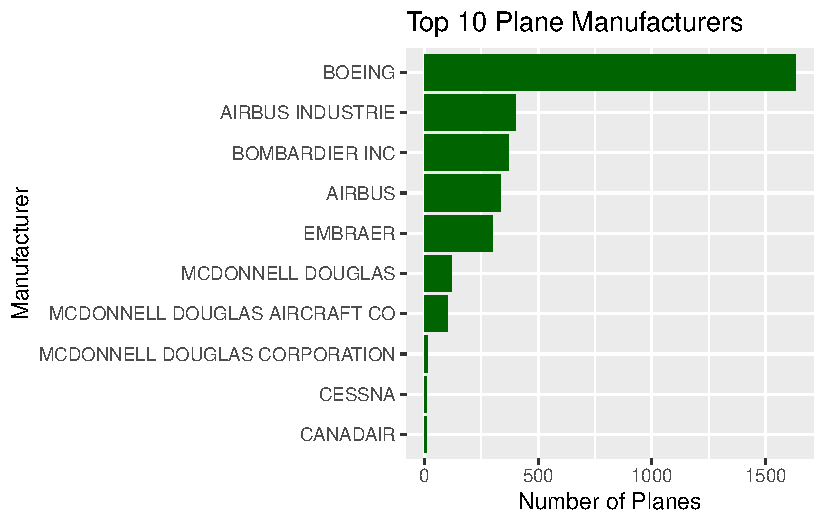
\includegraphics{6-StatistciallySpeaking_files/figure-pdf/unnamed-chunk-9-1.pdf}

The visualization above shows the top 10 plane manufacturers present in
the data-set. Boeing has the largest amount of planes with approximately
1750 planes, and Airbus has the second most with approximately 400
planes.

\begin{Shaded}
\begin{Highlighting}[numbers=left,,]
\FunctionTok{ggplot}\NormalTok{(planes, }\FunctionTok{aes}\NormalTok{(}\AttributeTok{x =}\NormalTok{ year)) }\SpecialCharTok{+}
  \FunctionTok{geom\_histogram}\NormalTok{(}\AttributeTok{binwidth =} \DecValTok{1}\NormalTok{, }\AttributeTok{fill =} \StringTok{"midnightblue"}\NormalTok{, }\AttributeTok{color =} \StringTok{"white"}\NormalTok{) }\SpecialCharTok{+}
  \FunctionTok{labs}\NormalTok{(}\AttributeTok{title =} \StringTok{"Distribution of Plane Manufacture Years"}\NormalTok{, }\AttributeTok{x =} \StringTok{"Year"}\NormalTok{, }\AttributeTok{y =} \StringTok{"Count"}\NormalTok{)}
\end{Highlighting}
\end{Shaded}

\begin{verbatim}
Warning: Removed 70 rows containing non-finite outside the scale range
(`stat_bin()`).
\end{verbatim}

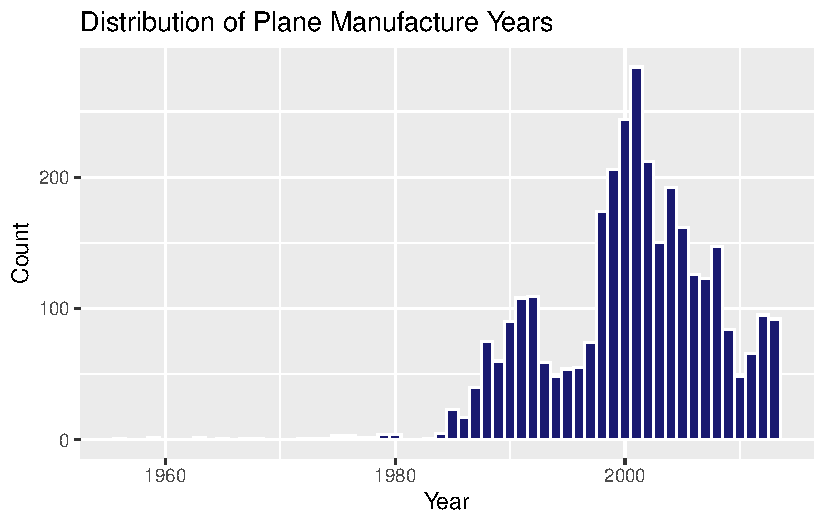
\includegraphics{6-StatistciallySpeaking_files/figure-pdf/unnamed-chunk-10-1.pdf}

This histogram shows the distribution of plane manufacture years, with
the majority of planes built between the mid-1990s and early 2000s.
There is a notable peak around the year 2000, indicating a surge in
plane production during that period.

\begin{Shaded}
\begin{Highlighting}[numbers=left,,]
\NormalTok{avg\_engines }\OtherTok{\textless{}{-}}\NormalTok{ planes }\SpecialCharTok{\%\textgreater{}\%}
  \FunctionTok{group\_by}\NormalTok{(engines) }\SpecialCharTok{\%\textgreater{}\%}
  \FunctionTok{summarise}\NormalTok{(}\AttributeTok{avg =} \FunctionTok{mean}\NormalTok{(engines, }\AttributeTok{na.rm =} \ConstantTok{TRUE}\NormalTok{))}

\CommentTok{\# Create the bar plot}
\FunctionTok{ggplot}\NormalTok{(avg\_engines, }\FunctionTok{aes}\NormalTok{(}\AttributeTok{x =} \FunctionTok{factor}\NormalTok{(engines), }\AttributeTok{y =}\NormalTok{ avg)) }\SpecialCharTok{+}
  \FunctionTok{geom\_bar}\NormalTok{(}\AttributeTok{stat =} \StringTok{"identity"}\NormalTok{, }\AttributeTok{fill =} \StringTok{"steelblue"}\NormalTok{) }\SpecialCharTok{+}
  \FunctionTok{labs}\NormalTok{(}\AttributeTok{title =} \StringTok{"Average Number of Engines per Plane"}\NormalTok{, }\AttributeTok{x =} \StringTok{"Number of Engines"}\NormalTok{, }\AttributeTok{y =} \StringTok{"Average"}\NormalTok{)}
\end{Highlighting}
\end{Shaded}

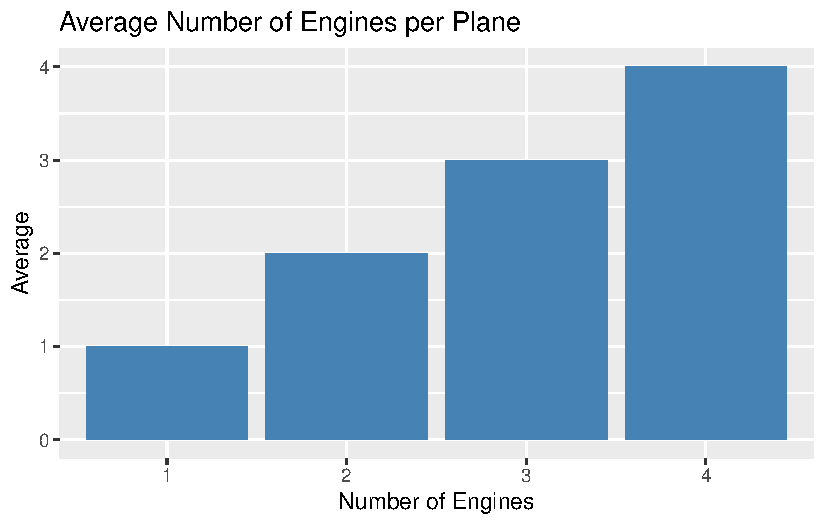
\includegraphics{6-StatistciallySpeaking_files/figure-pdf/unnamed-chunk-11-1.pdf}

\section{Analysis Approach Plan:}\label{analysis-approach-plan}

\textbf{Assumptions:} All variables are independent

The process of analysis will involve data cleaning after forming our
question, basic exploration of the data, comparison of certain datasets
with other datasets, visualization of the data, and an interpretation of
the data/results. Cleaning of the data will deal with tasks like
handling empty cells/columns and NA values. When it comes to exploratory
data analysis, we plan on using tools such as histograms and boxplots to
gain an understanding of the data and identify patterns and
relationships. The statistical analysis that we plan on performing with
the data will most likely involve making comparisons between groups to
compare airlines, times, and other metrics to make our overall claim.
For example, we might be comparing trends in time performance by weeks
or month between different airlines to gain a better understanding of
how differences in airlines affect delays. In terms of data
visualization, we will most likely be using line graphs for trends over
time when it comes to comparing flight time under different variables
and heatmaps/scatterplots for flight delays to help communicate our
findings. Finally, interpretation of the data will involve us answering
the proposed question by summarizing our statistics/findings as well as
through the presentation of graphical evidence.

\section{Alternative Strategies \& Back Up
Plan:}\label{alternative-strategies-back-up-plan}

As a backup idea, we are planning on seeing if there is any correlation
between the amount of delays present in the different airports. Our data
deals with the airports EWR, JFK, and LGA which are all different
airports within New York City. Our first question is to figure out if
the JFK airport has a different amount of delays compared to LGA or EWR
if there is a higher amount of precipitation in the JFK area. Although
all the airports are in New York, within the different areas of the
city, there can be different amounts of precipitation and rainfall that
occur. Our second question is to decide whether the different airports
have different models of planes and if the difference affects the
amounts of delays. For example if a plane is older or a different
configuration, does that lead to more delays due to cleaning or
maintenance? And lastly, our third question is whether the three
different airports have different airlines coming in and out and if
these differing airlines affect the amount of delays present on a given
day. For example, if Delta services one airport and not another, does
that increase or decrease the amount of total delays for an airport.
These questions can be further investigated if our first set of
questions are not approved or if we need more content to explore within
our project. These sets of backup questions will further explore the
flight data we have.




\end{document}
